\chapter{Artificial Neural Networks}\label{chp:3}

We saw in section \ref{limitations}, that the practical applicability of linear models with fixed basis functions is limited. One alternative is choosing a fixed number of \textcolor{blue}{\emph{adaptive basis functions}}. Here, basis functions are parametrized in a suitable way, and the parameters are adapted during the training in such a way such that the model explains (or “tuned” to) the given data. This approach can be carried out via using \textcolor{blue}{\emph{artificial neural networks}}, which we define in what follows.

\section{Fundamental Aspects}

\begin{definition}[Artificial Neural Network]
For a fixed $L \in \mathbb{N}$, let $n_0, \dots, n_L \in \mathbb{N}, W^{[\ell]} \in \mathbb{R}^{n_{\ell} \times n_{\ell -1}},$ and $b^{[\ell]} \in \mathbb{R}^{n_{\ell}}$ for all $\ell = 1, \dots, L$. Furthermore, let $g^{[\ell]}: \mathbb{R}^{n_{\ell}} \rightarrow \mathbb{R}^{n_{\ell}}$ for $\ell = 1, \dots, L$ be some functions. Then the function $f_{\theta} : \mathbb{R}^{n_0} \rightarrow \mathbb{R}^{n_L}$, which maps an \textcolor{blue}{\emph{input vector}} $x \in \mathbb{R}^{n_0}$ to
\begin{align}
    &f_{\theta}(x) := a^{[L]}, \quad \text{where}\\
    &a^{[0]} := x,\\
    &z^{[\ell]} := W^{[\ell]} a^{[\ell-1]} + b^{[\ell]},\\
    &a^{[\ell]} := g^{[\ell]}(z^{[\ell]}), \Biggr\} \quad \ell = 1, \ldots, L
    \label{eqn:29}
\end{align}

is called an \textcolor{blue}{\emph{artificial neural network}} with \textcolor{blue}{\emph{parameters}} $\theta = (W^{[1]}, b^{[1]}, \ldots, W^{[L]}, b^{[L]})$ and \textcolor{blue}{\emph{activation functions}} $g^{[1]}, \ldots, g^{[L]}$. The matrices $W^{[1]}, \ldots, W^{[L]}$ are called \textcolor{blue}{\emph{weight matrices}}, and the vectors $b^{[1]}, \ldots, b^{[L]}$ are called \textcolor{blue}{\emph{bias vectors}} of $f$.\\

For fixed $x \in \mathbb{R}^n_0$ and $\ell \in \{1, \ldots, L\}$, we call $z^{[\ell]} \in \mathbb{R}^{n_{\ell}}$ \textcolor{blue}{\emph{(net) input vector)}} and $a^{[\ell]} \in \mathbb{R}^{n_{\ell}}$ the \textcolor{blue}{\emph{activation vector)}} in the $\ell$-th layer, where $n_{\ell}$ is the \textcolor{blue}{\emph{width)}} of the $\ell$-th layer. Finally, $f_{\theta}(x)=a^{[L]}$ is the \textcolor{blue}{\emph{output vector)}}, and $L$ is called the \textcolor{blue}{\emph{depth)}} of $f_{\theta}$.
\end{definition}

\begin{figure}[h!]
    \centering
    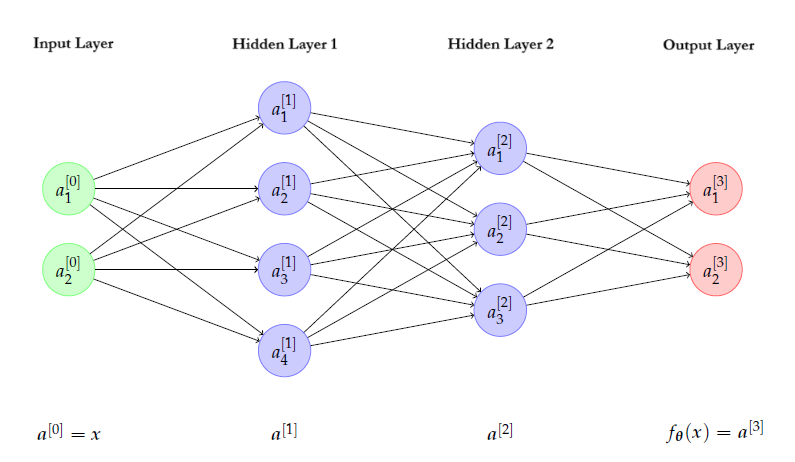
\includegraphics[width=\textwidth]{images/figure6.png}
    \caption{Example of an artificial neural network with two hidden layers.}
    \label{fig:6}
\end{figure}

\begin{remark}[Nonlinearity]
The vectors $a^{[0]}, \ldots, a^{[L]}$ and $z^{[1]}, \ldots, z^{[L]}$ defined in \ref{eqn:29} are, like $f_{\theta}$, functions of the input vector $x$. For simplicity, we usually omit this dependency in our notation as long as the context is clear. Nevertheless, we can understand $f_{\theta}$ as a composition of several linear and nonlinear functions. For example, for $L=1$ we have

\begin{equation}
    f_{\theta}(x) = g^{[1]}(W^{[1]}x + b^{[1]}),
    \label{eqn:30}
\end{equation}\\

meaning that $f_{\theta}$ is a composition of $g^{[1]}$ with $z^{[1]} = W^{[1]}x + b^{[1]}$. Also for $L=2$ we obtain a function

\begin{equation}
    f_{\theta}(x) = g^{[2]}(W^{[2]}(g^{[1]}(W^{[1]}x + b^{[1]})) + b^{[2]}),
    \label{eqn:31}
\end{equation}\\
and the process continues in the same way for $L \geq 3$.\\

In general at least some of the functions $g^{[\ell]}$ are chosen to be nonlinear. If this was not the case, then $f_{\theta}$, as a composition of linear functions, would also be linear. The additional and more complex structure \ref{eqn:29} would therefore have no advantage over a simple representation of the form $f_{\theta}(x) = Wx + b$ with $W \in \mathbb{R}^{n_L \times n_0}$ and $b \in \mathbb{R}^{n_L}$ (as every affine-linear function can be represented in such a way).

\end{remark}

\begin{remark}[Scalar Activation Functions]
The activation function $g^{[\ell]}: \mathbb{R}^{n_{\ell}} \rightarrow \mathbb{R}^{n_{\ell}}$ can often be interpreted as a component-wise application of a real function from $\mathbb{R}$ to $\mathbb{R}$. In this case, unless stated differently, for a scalar function $g^{[\ell]}: \mathbb{R} \rightarrow \mathbb{R}$, we define $g^{[\ell]}(z) \in \mathbb{R}^{n_{\ell}}$ as a component-wise application of $g^{[\ell]}$ to $z \in \mathbb{R}^{n_{\ell}}$,

\begin{equation}
    g^{[\ell]}(z) := \begin{pmatrix}
    g^{[\ell]}(z_1) \\
    \vdots \\
    g^{[\ell]}(z_{n_\ell})
    \end{pmatrix}.
    \label{eqn:32}
\end{equation}

\end{remark}

When defining a neural network, we decide on the type of activation functions that we use.
Below we give a few example of commonly used activation functions.

\begin{example}[Typical Activation Functions]
Depending on the context and goal of the problem, we can use any of the below activation functions (see Figure \ref{fig:7}) while defining the neural network:

\begin{figure}[h!]
    \centering
    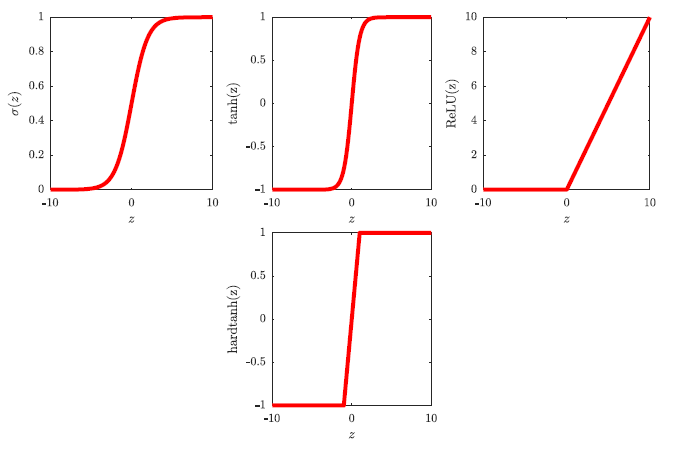
\includegraphics[width=0.8\textwidth]{images/figure7.png}
    \caption{Typical Activation Functions}
    \label{fig:7}
\end{figure}

\begin{itemize}
    \item \textcolor{blue}{\emph{Sigmoid function}}: Commonly used in the output layer of a binary classification task, as it maps values to the range $(0, 1)$, representing probabilities. Suitable when the model needs to output probabilities or interpret values as likelihoods, but it can suffer from vanishing gradients.\cite{hochreiter1997lstm, rumelhart1986learning}
    \begin{equation}
        \sigma: \mathbb{R} \to (0,1), \quad \sigma(z) := \frac{1}{1+e^{-z}}
        \label{eqn:33}
    \end{equation}
    
    \item \textcolor{blue}{\emph{ReLU (Rectified Linear Unit) function}}: It ensures sparsity by retaining only positive activations, which not only introduces non-linearity but also improves computational efficiency and helps avoid the vanishing gradient problem.\cite{nair2010relu}
    \begin{equation}
        \text{ReLU}(z): \mathbb{R} \to \mathbb{R}_{\geq 0}, \quad \text{ReLU}(z) := \max(0, z)
        \label{eqn:34}
    \end{equation}
    
    \item \textcolor{blue}{\emph{Hyperbolic Tangent (tanh) function}}: Preferred in hidden layers when inputs are zero-centered, as it maps the input in the range $(-1, 1)$, which helps faster convergence during training. It has more efficient gradient flow than sigmoid function.
    \begin{equation}
        \text{tanh}: \mathbb{R} \to (-1,1), \quad \text{tanh}(z) := \frac{e^z-e^{-z}}{e^z+e^{-z}}
        \label{eqn:35}
    \end{equation}
    
    \item \textcolor{blue}{\emph{Hard hyperbolic tangent (hardtanh) function}}: Provides a faster approximation of the traditional tanh function, maintaining a balance between non-linearity and computational simplicity.
    \begin{equation}
        \text{hardtanh}(z): \mathbb{R} \to [-1,1], \quad \text{hardtanh}(z) := \max(-1, \min(1,z))
        \label{eqn:36}
    \end{equation}
    
    \item \textcolor{blue}{\emph{Identity function}}: While it does not introduce non-linearity, it is occasionally used in skip connections or output layers when no transformation is needed.
    \begin{equation}
        \text{id}(z): \mathbb{R} \to \mathbb{R}, \quad \text{id}(z) := z
        \label{eqn:37}
    \end{equation}
    
    \item \textcolor{blue}{\emph{Softmax function}}: Typically applied at the output layer for multi-class classification tasks, converting raw scores into normalized probabilities.
    \begin{equation}
        \text{softmax}(z) : \mathbb{R}^n \to \mathbb{R}^n, \quad \text{softmax}(z)_j := \frac{e^{z_j}}{\sum_{j=1}^n e^{z_j}}
        \label{eqn:38}
    \end{equation}
\end{itemize}

\end{example}

\section{Multiclass Classification}
Assume that, in contrast to binary classification, we have not only two but $K$ different classes that we want to assign to elements $x \in \mathcal{X}$ of the sample space. Thus, we have the set $\{0, \ldots, K-1\}$ of $K$ different labels and we seek a \textcolor{blue}{\emph{hypothesis}} of the form $h_{\theta}: \mathbb{R}^d \rightarrow \{0, \ldots, K-1\}$. We realize this approach via the \textcolor{blue}{\emph{One-Hot encoding}}
\begin{equation}
    \{0, \ldots, K-1\} \rightarrow \mathbb{R}^K, \quad k \mapsto e_{k+1}
    \label{eqn:39}
\end{equation}

where $e_{k+1}$ denotes the $(k+1)$-st unit vector. We map every label $y^{(i)} \in \{0, \ldots, K-1\}$ of an element of the training dataset to the corresponding unit vector:

\begin{equation}
    y^{(i)} = e_{y^{(i)}+1} = \begin{pmatrix} 0 \\ \vdots \\ 0 \\ 1 \\ 0 \\ \vdots \\ 0 \end{pmatrix} \leftarrow \text{position } y^{(i)}+1 \in \mathbb{R}^K.
    \label{eqn:40}
\end{equation}

We then use the training data ${(x^{(1)}, y^{(1)}), \ldots, (x^{(m)}, y^{(m)})} \subseteq \mathcal{X} \times \{0, 1\}^K \subseteq \mathbb{R}^d \times \{0, 1\}^K$ and a neural network with input dimension $n_0 =d$ and output dimension $n_L = K$. Further, we determine the depth $L$, widths $n_1, \ldots, n_{L-1}$ of each layer, suitable activation functions $g^{[1]}, \ldots, g^{[L-1]}$ and choose $g^{[L]}:= \text{softmax}$ to be \ref{eqn:38}.

\begin{definition}[Softmax Loss]
The function
\begin{equation}
    \ell : \mathbb{R}^K \times \mathbb{R}^K_{>0} \rightarrow \mathbb{R}, \quad \ell(y, \hat{y}):= -\sum_{k=1}^{K}y_k \ln(\hat{y}_k)
    \label{eqn:41}
\end{equation}
is called \textcolor{blue}{\emph{softmax loss function}}.
\end{definition}

Using the softmax loss function, we will train an artificial neural network $f_{\theta}: \mathbb{R}^{n_0} \rightarrow \mathbb{R}^{n_L}$ by applying an optimization algorithm to the problem:
\begin{equation}
    \min_{\theta \in \Theta} - \frac{1}{m} \sum_{i=1}^{m} \sum_{k=1}^{K} y^{(i)}_k \ln(\hat{y}^{(i)_k}),
    \label{eqn:42}
\end{equation}

where $\theta = (W^{(1)}, b^{(1)}, \ldots, W^{(L)}, b^{(L)})$ ranges in the set $\Theta$ of parameters of the underlying artificial neural network. To identify the output of $f_{\theta}$ for the $i$-th training sample, we write $\hat{y}^{(i)}:= f_{\theta}(x^{(i)})$ in \ref{eqn:42}. For an object $x$ with unknown label and output $\hat{y} = f_{\theta}(x)$ we then assign the class
\begin{equation}
    h_{\theta}(x) = \left[ \argmax_{k=1, \ldots, K}\text{ } \hat{y}_k \right] - 1
    \label{eqn:43}
\end{equation}

The softmax function defined in \ref{eqn:38} represents a probability distribution over a discrete set. This makes it particularly suitable for the role of the output activation function $g^{[L]}$ for multiclass
classification. For a fixed input vector $x \in \mathbb{R}^d$ and the associated input vector $z^{[L]}$ of the $L$-th layer (output layer), we interpret
\begin{equation}
    \hat{y}_k = \text{softmax}(z^{[L]})_k = \mathcal{D}_{\text{Mod}}(y = k - 1 \mid x; \theta),
    \label{eqn:44}
\end{equation}

which explains why we choose the class with the highest probability in \ref{eqn:43}.\\

For $L=1$ and $z^{[1]} = (-(w^\top x + b),0)$, we obtain
% Requires: \usepackage{amsmath}
\begin{equation}
\hat{y} = \text{softmax}(z^{[L]}) = \left(1 - \sigma(w^\top x + b), \sigma(w^\top x + b)\right)
\label{eqn:45}
\end{equation}

and we see that the Bernoulli distribution \ref{eqn:3} arises as a particular case of \ref{eqn:44}. In particular, logistic regression \ref{eqn:7} is a very special instance of the multiclass classification (with $L = 1$ and \ref{eqn:38} as an output activation function) given by \ref{eqn:43}.

\begin{remark}[Maximum Likelihood Interpretation]
As for the cross entropy loss for binary classification, the softmax loss for multiclass classification can be derived via a maximum likelihood approach, where the statistical model is the family of distributions on $\mathcal{X} \times \{0, 1\}^K \subseteq \mathbb{R}^d \times \{0, 1\}^K$ given by \ref{eqn:44}. Using the vector $y \in \{e_1, \ldots, e_K\} \subseteq \mathbb{R}^K$, which is a one-hot encoded label $y \in \{0, \ldots, K-1\}$, we write \ref{eqn:44} as
\begin{equation}
    \mathcal{D}_{\text{Mod}}(y|x;\theta) = \mathcal{D}_{\text{Mod}}(y|x;\theta) := \prod_{k=1}^{K} [f_{\theta}(x)_{k}]^{y_k}
    \label{eqn:46}
\end{equation}
Then
\begin{equation}
    \mathcal{L}(\theta) = -\ln \mathcal{D}_{\text{Mod}}(S ; \theta) = -\ln \prod_{i=1}^{m} \prod_{k=1}^{K} \left[ f_\theta(x^{(i)})_k \right]^{y_k^{(i)}} = - \sum_{i=1}^{m} \sum_{k=1}^{K} y_k^{(i)} \ln f_\theta(x^{(i)})_k
    \label{eqn:47}
\end{equation}
is a negative log likelihood function, where the inner sum corresponds exactly to $\ell(y^{(i)}, f_{\theta}(x^{(i)}))$ from \ref{eqn:41}.
\end{remark}

\begin{figure}[h!]
    \centering
    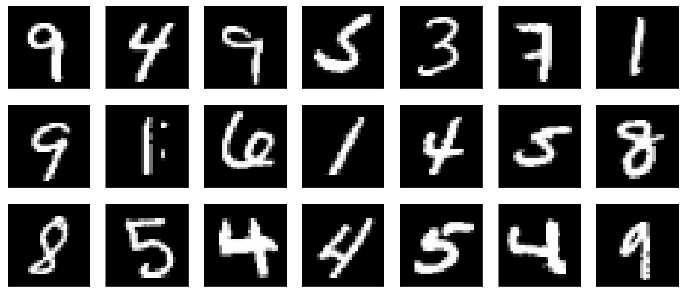
\includegraphics[width=\textwidth]{images/figure8.png}
    \caption{Random sampled objects from the MNIST dataset}
    \label{fig:8}
\end{figure}

\begin{example}[MNIST]
A dataset often used as a benchmark in the context of multiclass classification is the MNIST dataset (\cite{lecun1998mnist, lecun1998gradient}), containing over $60000$ training examples $(x^{(i)}, y^{(i)}) \in \mathbb{R}^{28 \times 28} \times \{0, \ldots, 9\}$. Every object $x^{(i)}$ is a grayscale image of a handwritten digit (Figure \ref{fig:8}) and the associated label $y^{(i)}$ corresponds exactly to the respective digit. In order to use the images $x^{(i)}$ (available as matrices) as an input for a neural network, they must be
vectorized (usually row-wise), such that we have an input dimension of $n_0 = 28^2 = 784$ and $n_L = 10$ as output dimension. In this example we use a neural network with depth $L=3$ and two hidden layers of width $n_1 = 100$ and $n_2 = 50$. Additionally, we apply \textcolor{blue}{\emph{batch normalization}} and \textcolor{blue}{\emph{dropout}}, two techniques allowing for a more efficient training and improving the model
performance on unseen data. We will later discuss these techniques in detail. With a sufficient number of gradient steps optimizing the problem \ref{eqn:42}, we can determine the parameters $\hat{\theta} = (W^{[1]}, b^{[1]}, W^{[2]}, b^{[2]}, W^{[3]}, b^{[3]})$, and obtain a classification accuracy of $98.37\%$ on the training data and $98.38\%$ on $10000$ unseen test images. IN Figure \ref{fig:9}, we visualize a subset of rows of the matrix $W^{[1]}$ after training. There we can see that some rows extract certain patterns from the input data, like line segments with a certain orientation on fixed positions in the image. The activation vector $a^{[1]}$ for a fixed input x thus contains information about the presence (or absence) of these simple geometric patterns. These information are combined in the second hidden layer to detect more complex patterns in the input images, which are encoded in the activation vector $a^{[2]}$. Based on these extracted patterns, the output layer then assigns the probability of the image belonging to each class.
\end{example}

\begin{figure}[h!]
    \centering
    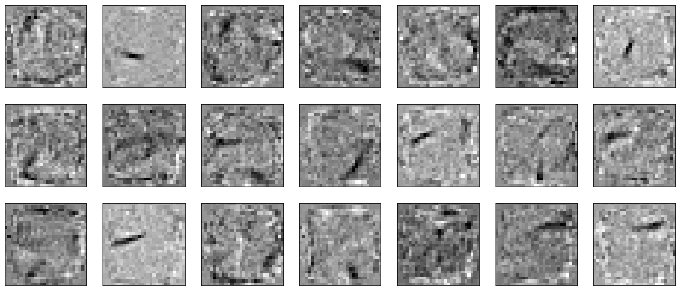
\includegraphics[width=\textwidth]{images/figure9.png}
    \caption{
    Subset of rows of the weight matrix $W^{[1]}$.The length of each row is equal to the input dimension $n_0 = 784$. Here, the rows are displayed as $28 \times 28$ grayscale images, which is the original format of the images $x^{(i)}$. Light pixels tend to correspond to positive entries, while dark pixels corresponds to negative entries and gray pixels to small absolute values.
    }
    \label{fig:9}
\end{figure}

\section{Error Backpropagation}
In order to solve the optimization problem
\begin{equation}
    \hat{\theta} \in \argmin_{\theta \in \Theta} \mathcal{J}(\theta) = \argmin_{\theta \in \Theta} \frac{1}{m} \sum_{i=1}^{m} \ell(y^{(i)}, f_\theta(x^{(i)}))
    \label{eqn:48}
\end{equation}

for a loss function $\ell$ and an artificial neural network $f_{\theta}$ with a \emph{gradient descent method}, we need to compute partial derivatives of $\ell(y^{(i)}, f_\theta(x^{(i)}))$ along the parameters $\hat{\theta} = (W^{[1]}, b^{[1]}, \ldots, W^{[L]}, b^{[L]})$. To compute a derivative of $\mathcal{J}$ (for a fixed training data set) we simply have to sum and divide by $m$ the derivatives of $\ell(y^{(i)}, f_\theta(x^{(i)}))$. In the following, we derive the \textcolor{blue}{\emph{backpropagation}} algorithm used for this purpose (see for example \cite[section 6.5]{goodfellow2016deep}, \cite[section 5.3]{bishop2006pattern}).

\subsection{Derivatives for one Object on Parameter Basis}

\begin{lemma}[Partial derivatives with respect to parameters]\label{partial_derivative}
Let $f_{\theta}: \mathbb{R}^{n_0} \rightarrow \mathbb{R}^{n_L}$ be an artificial neural network with parameters $\hat{\theta} = (W^{[1]}, b^{[1]}, \ldots, W^{[L]}, b^{[L]}), \ell: \mathbb{R}^{n_L} \times \mathbb{R}^{n_L} \rightarrow \mathbb{R}$, a loss function, and $(x, y) \in \mathbb{R}^{n_0} \times \mathbb{R}^{n_L}$. If we define for all $\ell \in \{1, \ldots, L\}$ and all $j \in \{1, \ldots, n_{\ell}$
\begin{equation}
    \delta_j^{[\ell]} := \frac{\partial \ell (y, f_\theta (x))}{\partial z_j^{[\ell]}} ,
    \label{eqn:49}
\end{equation}

then it holds
\begin{equation}
    \frac{\partial \ell(y, f_\theta(x))}{\partial w_{ji}^{[\ell]}} = \delta_j^{[\ell]} a_i^{[\ell-1]}
    \quad \text{and} \quad
    \frac{\partial \ell(y, f_\theta(x))}{\partial b_j^{[\ell]}} = \delta_j^{[\ell]}.
    \label{eqn:50}
\end{equation}
\end{lemma}\\

\textbf{\emph{Proof.}} The value of the objective function $\ell(y, f_\theta(x))$ depends exclusively on the weights $w_{ji}^{[\ell]}$ via the relation
\begin{equation}
z_j^{[\ell]} = \sum_{i=1}^{n_{\ell-1}} w_{ji}^{[\ell]} a_i^{[\ell-1]} + b_j^{[\ell]}.
\label{eqn:51}
\end{equation}

Therefore, we can apply the chain rule for the derivative and obtain
\begin{equation}
\frac{\partial \ell(y, f_\theta(x))}{\partial w_{ji}^{[\ell]}} = \frac{\partial \ell(y, f_\theta(x))}{\partial z_j^{[\ell]}} \cdot \frac{\partial z_j^{[\ell]}}{\partial w_{ji}^{[\ell]}} = \delta_j^{[\ell]} a_i^{[\ell-1]}.
\label{eqn:52}
\end{equation}

Analogously, we obtain the derivative with respect to $b_j^{[\ell]}$ with the difference that $\frac{\partial z_j^{[\ell]}}{\partial b_j^{[\ell]}} = 1$.\\

Lemma \ref{partial_derivative} states that we can determine the derivatives of $\ell(y, f_{\theta}(x))$ with respect to the weights and biases with only little effort, if we know the derivatives of the respective inputs.

\begin{theorem}[Backpropagation]\label{backpropagation}
Let $f_{\theta}: \mathbb{R}^{n_0} \rightarrow \mathbb{R}^{n_L}$ be an artificial neural network with parameters $\hat{\theta} = (W^{[1]}, b^{[1]}, \ldots, W^{[L]}, b^{[L]})$, loss function $\ell: \mathbb{R}^{n_L} \times \mathbb{R}^{n_L} \rightarrow \mathbb{R}$ and $(x, y) \in \mathbb{R}^{n_0} \times \mathbb{R}^{n_L}$. Furthermore, let the activation functions $g^{[1]}, \ldots, g^{[L-1]}: \mathbb{R} \rightarrow \mathbb{R}$ be defined component-wise. Then it holds for every $j \in \{1, \ldots, n_L\}$
\begin{equation}
    \delta_j^{[L]} = \sum_{k=1}^{n_L} \frac{\partial \ell(y, f_\theta(x))}{\partial a_k^{[L]}} \cdot \frac{\partial a_k^{[L]}}{\partial z_j^{[L]}}
    \label{eqn:53}
\end{equation}

and further for every $\ell \in \{1, \ldots, L-1\}$ and every $j \in \{1, \ldots, n_{\ell}\}$
\begin{equation}
    \delta_j^{[\ell]} = g^{[\ell]'}(z_j^{[\ell]}) \sum_{k=1}^{n_{\ell+1}} \delta_k^{[\ell+1]} w_{kj}^{[\ell+1]}.
    \label{eqn:54}
\end{equation}
\end{theorem}\\

\textbf{\emph{Proof.}} The first claim \ref{eqn:53} follows directly from the definition \ref{eqn:49} and the chain rule because the function $\ell(y, f_{\theta}(x))$ only depends on $z_j^{[L]}$ through $a^{[L]}$. Thus
\begin{equation}
    \delta_j^{[L]} = \frac{\partial \ell(y, f_\theta(x))}{\partial z_j^{[L]}} = \underbrace{\frac{\partial \ell(y, f_\theta(x))}{\partial a^{[L]}}}_{1 \times n_L} \cdot \underbrace{\frac{\partial a^{[L]}}{\partial z_j^{[L]}}}_{n_L \times 1} = \sum_{k=1}^{n_L} \frac{\partial \ell(y, f_\theta(x))}{\partial a_k^{[L]}} \cdot \frac{\partial a_k^{[L]}}{\partial z_j^{[L]}}.
    \label{eqn:55}
\end{equation}

For the second claim, we can also apply the chain rule as follows:
\begin{equation}
    \begin{aligned}
    \delta_{j}^{[\ell]} &= \frac{\partial \ell (y, f_{\theta} (x))}{\partial z_{j}^{[\ell]}} = \underbrace{\frac{\partial \ell (y, f_{\theta} (x))}{\partial z^{[\ell+1]}}}_{1 \times n_{\ell + 1}} \cdot \underbrace{\frac{\partial z^{[\ell+1]}}{\partial z_{j}^{[\ell]}}}_{n_{\ell + 1} \times 1}\\
    &= \sum_{k=1}^{n_{\ell+1}} \underbrace{\frac{\partial \ell (y, f_\theta (x))}{\partial z_{k}^{[\ell+1]}}}_{\delta_k^{[\ell + 1]}} \cdot \frac{\partial z_{k}^{[\ell+1]}}{\partial z_{j}^{[\ell]}} = \sum_{k=1}^{n_{\ell+1}} \delta_{k}^{[\ell+1]} \cdot \underbrace{\frac{\partial z_{k}^{[\ell+1]}}{\partial a_{j}^{[\ell]}}}_{=w_{kj}^{[\ell + 1]}} \cdot \underbrace{\frac{\partial a_{j}^{[\ell]}}{\partial z_{j}^{[\ell]}}}_{=g^{[\ell]'} \left( z_{j}^{[\ell]} \right)}\\
    &= g^{[\ell]'} \left( z_{j}^{[\ell]} \right) \sum_{k=1}^{n_{\ell+1}} \delta_{k}^{[\ell+1]} w_{kj}^{[\ell+1]}.
    \end{aligned}
    \label{eqn:56}
\end{equation}

\begin{remark}[Activation functions in the output layer]
In Theorem \ref{backpropagation}, we assumed that the activation functions $g^{[1]}, \ldots, g^{[L-1]}: \mathbb{R} \rightarrow \mathbb{R}$ are defined component-wise, while we intentionally
omitted this assumption for the activation function $g^{[L]}$ in the last layer. The reason for that is that the function $\text{softmax }: \mathbb{R}^n \rightarrow \mathbb{R}^n$ typically used as an activation in the last layer is not defined component-wise. If, in contrast, $g^{[L]}: \mathbb{R} \rightarrow \mathbb{R}$ is also defined component-wise, we obtain a simpler representation of (\ref{eqn:53}),
\begin{equation}
    \delta_j^{[L]} = \frac{\partial \ell(y, f_\theta(x))}{\partial a_j^{[L]}} \cdot \frac{\partial a_j^{[L]}}{\partial z_j^{[L]}} = g^{[L]'} \left( z_{j}^{[L]} \right) \cdot \frac{\partial \ell(y, f_\theta(x))}{\partial a_j^{[L]}}
    \label{eqn:57}
\end{equation}
\end{remark}

\subsection{Vectorized Derivatives for one Object}
With Lemma \ref{partial_derivative} and Theorem \ref{backpropagation} we are now able to compute the derivatives of $\ell(y, f_\theta(x))$ with respect to $w_ji^{[\ell]}$ and $b_j^{[\ell]}$ for a fixed training example $(x, y)$. To achieve a more efficient implementation of the backpropagation it is useful to compute these derivatives not with respect to every single parameter but directly with respect to the whole weight matrix $W^{[\ell]}$ and bias vector $b^{[\ell]}$. For that, we \emph{vectorize} the derivation process.

\begin{definition}[Error]
For a fixed $(x, y) \in \mathbb{R}^{n_0} \times \mathbb{R}^{n_L}$ and $\ell \in \{1, \ldots, L\}$ we define
\begin{equation}
    \delta^{[\ell]} := \begin{pmatrix}
        \delta_1^{[\ell]} \\ \vdots \\ \delta_{n_{\ell}}^{[\ell]}
    \end{pmatrix} \in \mathbb{R}^{n_{\ell}}
    \label{eqn:58}
\end{equation}
as the \textcolor{blue}{\emph{error}} of the $\ell$-th layer.
\end{definition}

To calculate $\delta^{[\ell]}$, we need to distinguish the two cases $\ell = L$ and $\ell < L$, as we already did in Theorem \ref{backpropagation}. In the case $\ell = L$ we can directly expand the definition to

\begin{equation}
    \begin{aligned}
    \delta^{[L]\top} &= \frac{\partial \ell(y, f_\theta(x))}{\partial z^{[L]}} = \frac{\partial \ell(y, f_\theta(x))}{\partial a^{[L]}} \cdot \frac{\partial a^{[L]}}{\partial z^{[L]}}\\
    &= \underbrace{\begin{pmatrix}
        \frac{\partial \ell(y, f_\theta(x))}{\partial a_1^{[L]}} \cdots \frac{\partial \ell(y, f_\theta(x))}{\partial a_{n_L}^{[L]}}
    \end{pmatrix}}_{1 \times n_L} \underbrace{\begin{pmatrix}
        \frac{\partial a_1^{[L]}}{\partial z_1^{[L]}} & \cdots & \frac{\partial a_1^{[L]}}{\partial z_{n_L}^{[L]}}\\
        \vdots & \ddots & \vdots\\
        \frac{\partial a_{n_L}^{[L]}}{\partial z_1^{[L]}} & \cdots & \frac{\partial a_{n_L}^{[L]}}{\partial z_{n_L}^{[L]}}
    \end{pmatrix}}_{n_L \times n_L}
    \end{aligned}
    \label{eqn:59}
\end{equation}

By analogy with (\ref{eqn:57}) we obtain,
\begin{equation}
    \delta^{[L]} = g^{[L]'} \left( z^{[L]} \right) \odot \left[ \frac{\partial \ell (y, f_\theta(x))}{\partial a^{[L]}}  \right]^\top = g^{[L]'} \left( z^{[L]} \right) \odot \triangledown_{a^{[L]}} \ell(y, f_\theta(x))
    \label{eqn:60}
\end{equation}

for a component-wise defined $g^{[L]}: \mathbb{R} \rightarrow \mathbb{R}$, where $g^{[L]'}: \mathbb{R} \rightarrow \mathbb{R}$ is also applied component-wise to $z^{[L]}$. Here, with $\odot$ we denote the component-wise multiplication of two vectors. Note that in this case $\partial a^{[L]} / \partial z^{[L]}$ is a diagonal matrix with entries $g^{[L]'} \left( z^{[L]} \right), j= 1, \ldots, n_L$.

\begin{remark}
In several cases of interest (e.g., when $g^{[L]}$ is the softmax function (\ref{eqn:38})) it holds
\begin{equation}
    \delta^{[L]} = f_\theta(x) - y
    \label{eqn:61}
\end{equation}
\end{remark}
\vspace{2em}
Now consider the second case $\ell < L$. With (\ref{eqn:54}) we can directly see that

\vspace{5em}
\textbf{TO BE CONTINUED...}


